\documentclass{article}
\usepackage[utf8]{inputenc}
\usepackage{listings}
\usepackage{graphicx}
\graphicspath{ {./images/} }
\usepackage[a4paper, total={6in, 8in}]{geometry}

\title{Approfondimento}

\author{Filmon Arefayne}
\date{Settembre 2019}

\begin{document}

\maketitle

\section{Introduzione}

Il progetto scelto approfondisce il design pattern \textbf{Command} in particolare si è incentrato nello sviluppo di un applicazione con interfaccia grafica che simula una SmartHome. In questa SmartHome si hanno tre telecomandi che rappresentano tre stanze (\textbf{Bedroom},\textbf{Kitchen} e \textbf{LivingRoom}) e per ogni stanza si hanno due Receiver  \textbf{Fan} e \textbf{Light} che devono poter rispondere ai comandi rispettivamente \textbf{Start/Stop} e \textbf{turnOn/turnOff}.
\\
Il problema consiste nella progettazione di una classe \textbf{SmartHomeRemote}, in grado di inoltrare richieste verso oggetti che saranno noti solo in fasi successive di sviluppo. Inoltre per l'implementazione della funzione \textbf{undo} è stato aggiunto uno oggetto \textbf{Stack} per mantenere in memoria le operazioni effettuate.
L'applicazione permette di selezionare la stanza e il comando da eseguire.L'ultimo comando eseguito viene mandato in output e una \textbf{JTextArea} permette di visualizzare lo status della SmartHome.Inoltre è possibile fare undo sulle ultime operazioni eseguite o resettare completamente l'applicazione.
\begin{figure}[ht]
\caption{L'applicazione in esecuzione}
\centering
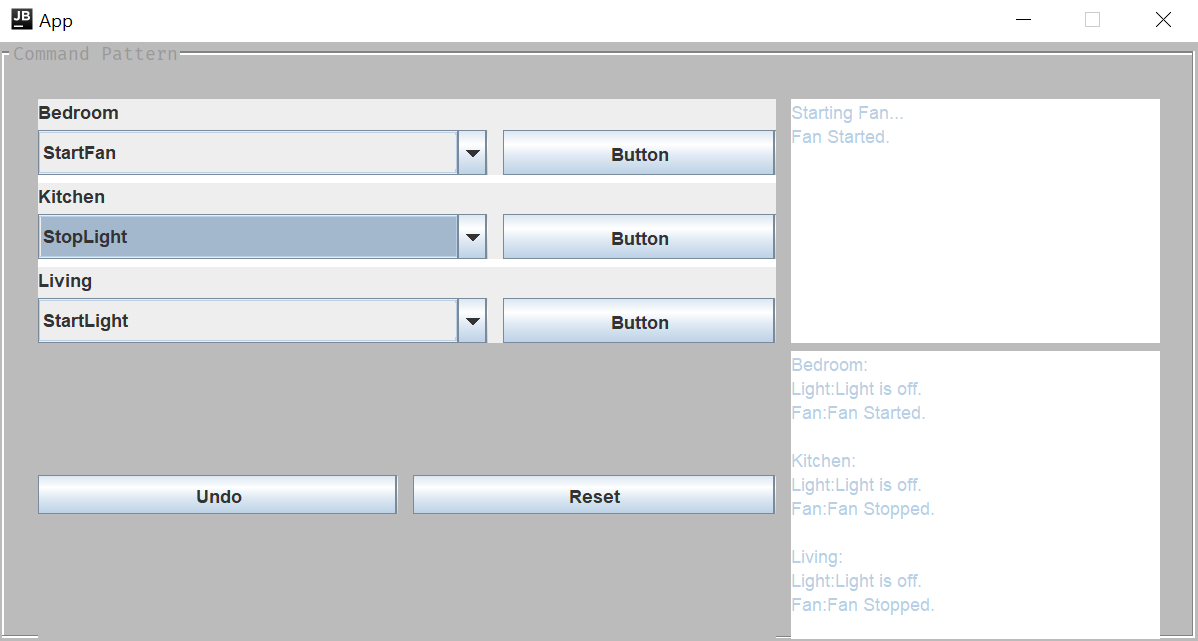
\includegraphics[width=\textwidth]{images/Approfondimento1.PNG}
\end{figure}

\section{Codice}

\begin{lstlisting}[language=Java]






// Command.java

package com.filmon.businesslogic;

public interface Command {
    public String execute();
    public String undo();
}








// SmartHomeRemote.java

package com.filmon.businesslogic;

public class SmartHomeRemote {
    private Command command;

    public void setCommand(Command command) {
        this.command = command;
    }

    public String buttonPressed() {
        return command.execute();
    }
    public String undoPressed() {
        return command.undo();
    }
}






// Fan.java

package com.filmon.businesslogic;

import java.util.Stack;

public class Fan {
    private boolean state = false;
    private Stack<Boolean> previousStates = new Stack<Boolean>();

    public String start() {
        previousStates.add(state);
        if(!state) {
            state = true;
            return status();
        }else
            return "Fan is unchanged";

    }
    public String stop() {
        previousStates.add(state);
        if(state) {
            state = false;
            return status();
        }else
            return "Fan is unchanged";

    }
    public String undo(){
        boolean ps;
        if(!previousStates.isEmpty()) {
            ps = previousStates.pop();
            if (ps == state) {
                return "Undoing nothing";
            } else {
                state = ps;
                return status();
            }
        }
        return "Undoing nothing";
    }
    public String status(){
        if(state){
            return "Fan Started.";
        }
        return "Fan Stopped.";
    }
}

// Light.java

package com.filmon.businesslogic;

import java.util.Stack;

public class Light {
    private boolean state = false;
    private Stack<Boolean> previousStates = new Stack<Boolean>();

    public String turnOn() {
        previousStates.add(state);
        if(!state) {
            state = true;
            return status();
        }else
            return "Light is unchanged";
    }

    public String turnOff() {
        previousStates.add(state);
        if(state) {
            state = false;
            return status();
        }else
            return "Light is unchanged";
    }
    public String undo(){
        boolean ps;
        if(!previousStates.isEmpty()) {
            ps = previousStates.pop();
            if (ps == state) {
                return "Undoing nothing";
            } else {
                state = ps;
                return status();
            }
        }
        return "Undoing nothing";
    }
    public String status(){
        if(state){
            return "Light is on.";
        }
        return "Light is off.";
    }
}

// StartFanCommand.java

package com.filmon.businesslogic;

public class StartFanCommand implements Command {
    private Fan fan;

    public StartFanCommand(Fan fan) {
        this.fan = fan;
    }
    @Override
    public String execute() {
        String temp;
        temp = "Starting Fan...\n";
        return temp + fan.start();
    }
    @Override
    public String undo() {
        String temp;
        temp = "Undoing...\n";
        return temp + fan.undo();
    }
}

// StopFanCommand.java

package com.filmon.businesslogic;

public class StopFanCommand implements Command{
    private Fan fan;

    public StopFanCommand(Fan fan) {
        this.fan = fan;
    }
    @Override
    public String execute() {
        String temp;
        temp = "Stopping Fan...\n";
        return temp + fan.stop();
    }
    @Override
    public String undo() {
        String temp;
        temp = "Undoing...\n";
        return temp + fan.undo();
    }
}

// TurnOnLightCommand.java

package com.filmon.businesslogic;

public class TurnOnLightCommand implements Command{
    private Light light;

    public TurnOnLightCommand(Light light) {
        this.light = light;
    }
    @Override
    public String execute() {
        String temp;
        temp = "Turning on Light...\n";
        return temp + light.turnOn();
    }
    @Override
    public String undo() {
        String temp;
        temp = "Undoing...\n";
        return temp + light.undo();
    }
}

// TurnOffLightCommand.java

package com.filmon.businesslogic;

public class TurnOffLightCommand implements Command {
    private Light light;

    public TurnOffLightCommand(Light light) {
        this.light = light;
    }
    @Override
    public String execute() {
        String temp;
        temp = "Turning off Light...\n";
        return temp + light.turnOff();
    }
    @Override
    public String undo() {
        String temp;
        temp = "Undoing...\n";
        return temp + light.undo();
    }
}

// App.java

package com.filmon;

import com.filmon.businesslogic.*;

import javax.swing.*;
import java.awt.event.ActionEvent;
import java.awt.event.ActionListener;
import java.util.Stack;

public class App {
    private JPanel panelMain;

    private JButton buttonBed;
    private JButton buttonKitchen;
    private JButton buttonLiving;

    private JComboBox<COMMAND> comboBoxBed;
    private JComboBox<COMMAND> comboBoxKitchen;
    private JComboBox<COMMAND> comboBoxLiving;

    private JButton buttonUndo;
    private JButton buttonReset;

    private JTextArea textAreaOutput;
    private JTextArea textAreaStatus;

    private Stack<SmartHomeRemote> shrs;
    private Light bedLight;
    private Fan bedFan;
    private Light kitchenLight;
    private Fan kitchenFan;
    private Light livingLight;
    private Fan livingFan;

    private SmartHomeRemote bedRemote;
    private SmartHomeRemote kitchenRemote;
    private SmartHomeRemote livingRemote;
    private enum COMMAND {
        StartLight,
        StopLight,
        StartFan,
        StopFan
    }
    public App() {
        reset();

        buttonBed.addActionListener(new ActionListener() {
            @Override
            public void actionPerformed(ActionEvent actionEvent) {
                textAreaOutput.setText(bedRemote.buttonPressed());
                shrs.add(bedRemote);
                update();
            }
        });
        buttonKitchen.addActionListener(new ActionListener() {
            @Override
            public void actionPerformed(ActionEvent actionEvent) {
                textAreaOutput.setText(kitchenRemote.buttonPressed());
                shrs.add(kitchenRemote);
                update();
            }
        });
        buttonLiving.addActionListener(new ActionListener() {
            @Override
            public void actionPerformed(ActionEvent actionEvent) {
                textAreaOutput.setText(livingRemote.buttonPressed());
                shrs.add(livingRemote);
                update();
            }
        });

        comboBoxBed.addItem(COMMAND.StartLight);
        comboBoxBed.addItem(COMMAND.StopLight);
        comboBoxBed.addItem(COMMAND.StartFan);
        comboBoxBed.addItem(COMMAND.StopFan);

        comboBoxKitchen.addItem(COMMAND.StartLight);
        comboBoxKitchen.addItem(COMMAND.StopLight);
        comboBoxKitchen.addItem(COMMAND.StartFan);
        comboBoxKitchen.addItem(COMMAND.StopFan);

        comboBoxLiving.addItem(COMMAND.StartLight);
        comboBoxLiving.addItem(COMMAND.StopLight);
        comboBoxLiving.addItem(COMMAND.StartFan);
        comboBoxLiving.addItem(COMMAND.StopFan);

        comboBoxBed.addActionListener(new ActionListener() {
            @Override
            public void actionPerformed(ActionEvent actionEvent) {
                Command command;
                switch (comboBoxBed.getSelectedIndex()){
                    case 0:
                        command = new TurnOnLightCommand(bedLight);
                        break;
                    case 1:
                        command = new TurnOffLightCommand(bedLight);
                        break;
                    case 2:
                        command = new StartFanCommand(bedFan);
                        break;
                    default:
                    case 3:
                        command = new StopFanCommand(bedFan);
                        break;
                }
                bedRemote.setCommand(command);
            }
        });
        comboBoxKitchen.addActionListener(new ActionListener() {
            @Override
            public void actionPerformed(ActionEvent actionEvent) {
                Command command;
                switch (comboBoxKitchen.getSelectedIndex()){
                    case 0:
                        command = new TurnOnLightCommand(kitchenLight);
                        break;
                    case 1:
                        command = new TurnOffLightCommand(kitchenLight);
                        break;
                    case 2:
                        command = new StartFanCommand(kitchenFan);
                        break;
                    default:
                    case 3:
                        command = new StopFanCommand(kitchenFan);
                        break;
                }
                kitchenRemote.setCommand(command);
            }
        });
        comboBoxLiving.addActionListener(new ActionListener() {
            @Override
            public void actionPerformed(ActionEvent actionEvent) {
                Command command;
                switch (comboBoxLiving.getSelectedIndex()){
                    case 0:
                        command = new TurnOnLightCommand(livingLight);
                        break;
                    case 1:
                        command = new TurnOffLightCommand(livingLight);
                        break;
                    case 2:
                        command = new StartFanCommand(livingFan);
                        break;
                    default:
                    case 3:
                        command = new StopFanCommand(livingFan);
                        break;
                }
                livingRemote.setCommand(command);
            }
        });
        comboBoxBed.setSelectedItem(COMMAND.StartLight);
        comboBoxKitchen.setSelectedItem(COMMAND.StartLight);
        comboBoxLiving.setSelectedItem(COMMAND.StartLight);

        textAreaOutput.setEnabled(false);
        textAreaStatus.setEnabled(false);
        buttonUndo.addActionListener(new ActionListener() {
            @Override
            public void actionPerformed(ActionEvent actionEvent) {
                SmartHomeRemote undoRemote;
                if (!shrs.isEmpty()){
                    undoRemote = shrs.pop();
                    textAreaOutput.setText(undoRemote.undoPressed());
                    update();
                }
            }
        });
        buttonReset.addActionListener(new ActionListener() {
            @Override
            public void actionPerformed(ActionEvent actionEvent) {
                reset();
                comboBoxBed.setSelectedItem(COMMAND.StartLight);
                comboBoxKitchen.setSelectedItem(COMMAND.StartLight);
                comboBoxLiving.setSelectedItem(COMMAND.StartLight);
            }
        });
    }
    private void reset(){
        shrs = new Stack<>();
        bedLight = new Light();
        kitchenLight = new Light();
        livingLight = new Light();

        bedFan = new Fan();
        kitchenFan = new Fan();
        livingFan = new Fan();

        bedRemote = new SmartHomeRemote();
        kitchenRemote = new SmartHomeRemote();
        livingRemote = new SmartHomeRemote();

        textAreaOutput.setText("");
        textAreaStatus.setText("");
    }
    private void update(){
        textAreaStatus.setText(
                "Bedroom: \n" +
                "Light:"+bedLight.status()+"\n"+
                "Fan:"+bedFan.status()+"\n\n"+
                "Kitchen: \n" +
                "Light:"+kitchenLight.status()+"\n"+
                "Fan:"+kitchenFan.status()+"\n\n"+
                "Living: \n" +
                "Light:"+livingLight.status()+"\n"+
                "Fan:"+livingFan.status()+"\n"
                );
    }
    public static void main(String[] args)  {

        JFrame frame = new JFrame("App");
        frame.setContentPane(new App().panelMain);
        frame.setDefaultCloseOperation(JFrame.EXIT_ON_CLOSE);
        frame.pack();
        frame.setVisible(true);
        frame.setResizable(false);
    }
}


\end{lstlisting}

\begin{figure}[ht]
\caption{Class Diagram dell'applicazione}
\centering
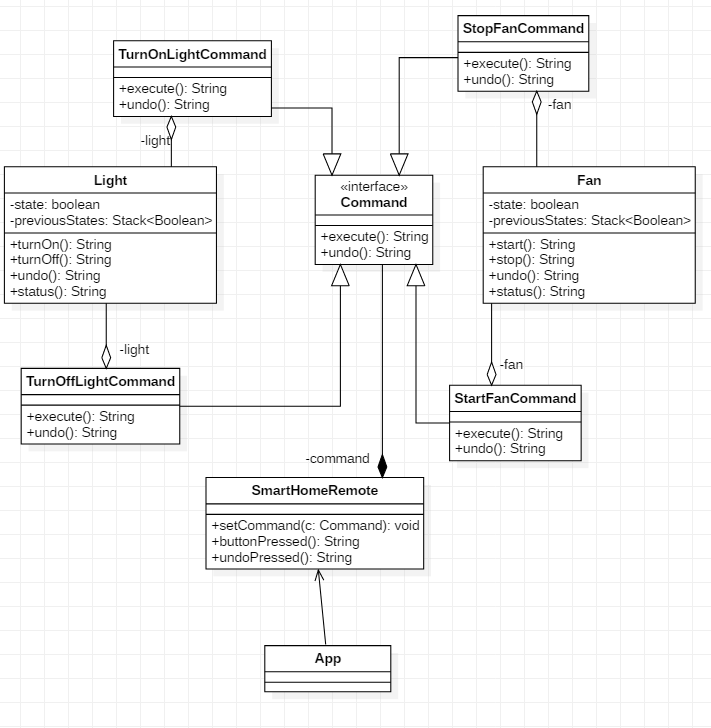
\includegraphics[width=\textwidth]{images/ApprofondimentoUML.PNG}
\end{figure}

\end{document}
